\documentclass[12pt, a4paper,reqno]{article}

\usepackage{amsmath}
\usepackage{amssymb}
\usepackage{graphicx}
\usepackage{float}
\usepackage{caption}
\usepackage{subcaption}
\usepackage{pdfpages}
\usepackage{minted}
\usepackage{color, soul}

\setlength{\parindent}{0pt}
\setlength{\parskip}{1em}


%
% Begin Document
%
\begin{document}

% TODO: Add date
% Cover Page

\includepdf[pages=-]{End_Assessment_Front_Page_HYXC3.pdf}


%
% Question 1
%
\section*{Question 1}

% Subsection 1(a)
\subsection*{1(a)}
With reference to the diagram of the basic \emph{logistic unit} on the following page:

The input vector $\mathbf{x}$ is the input to the \emph{logistic unit}.

Each input ${x}_i$ has an associated weight $\theta_i$. The weights are set to a random value prior to \emph{training}. The \emph{training} process determines these weights.

The product of each input $x_i$ and weight $\theta_i$ is summed to produce a weighted sum $z$.

The output, $h_\theta(x)$, is the the non-linear \emph{activation function}, $h$, applied to $z$.

% Subsection 1(b)
\subsection*{1(b)}

Consider the diagram of Question 1(a).

The weighted sum of the inputs, $z$, is:

\begin{equation}
z = \sum_{j=1}^{n}\theta_j x_j = \theta^T x
\end{equation}

where $x_i$ is the $i^{th}$ element of input vector $\mathbf{x}$ of length $n$, and $\theta_i$ is the associated \emph{weight}. 

And, the output from the \emph{logistic unit}, $h_\theta(x)$, is:

\begin{equation}
h_\theta(x) = h(z)
\end{equation}

where $h$ is a non-linear \emph{activation function}.

% Subsection 1(a) - diagram
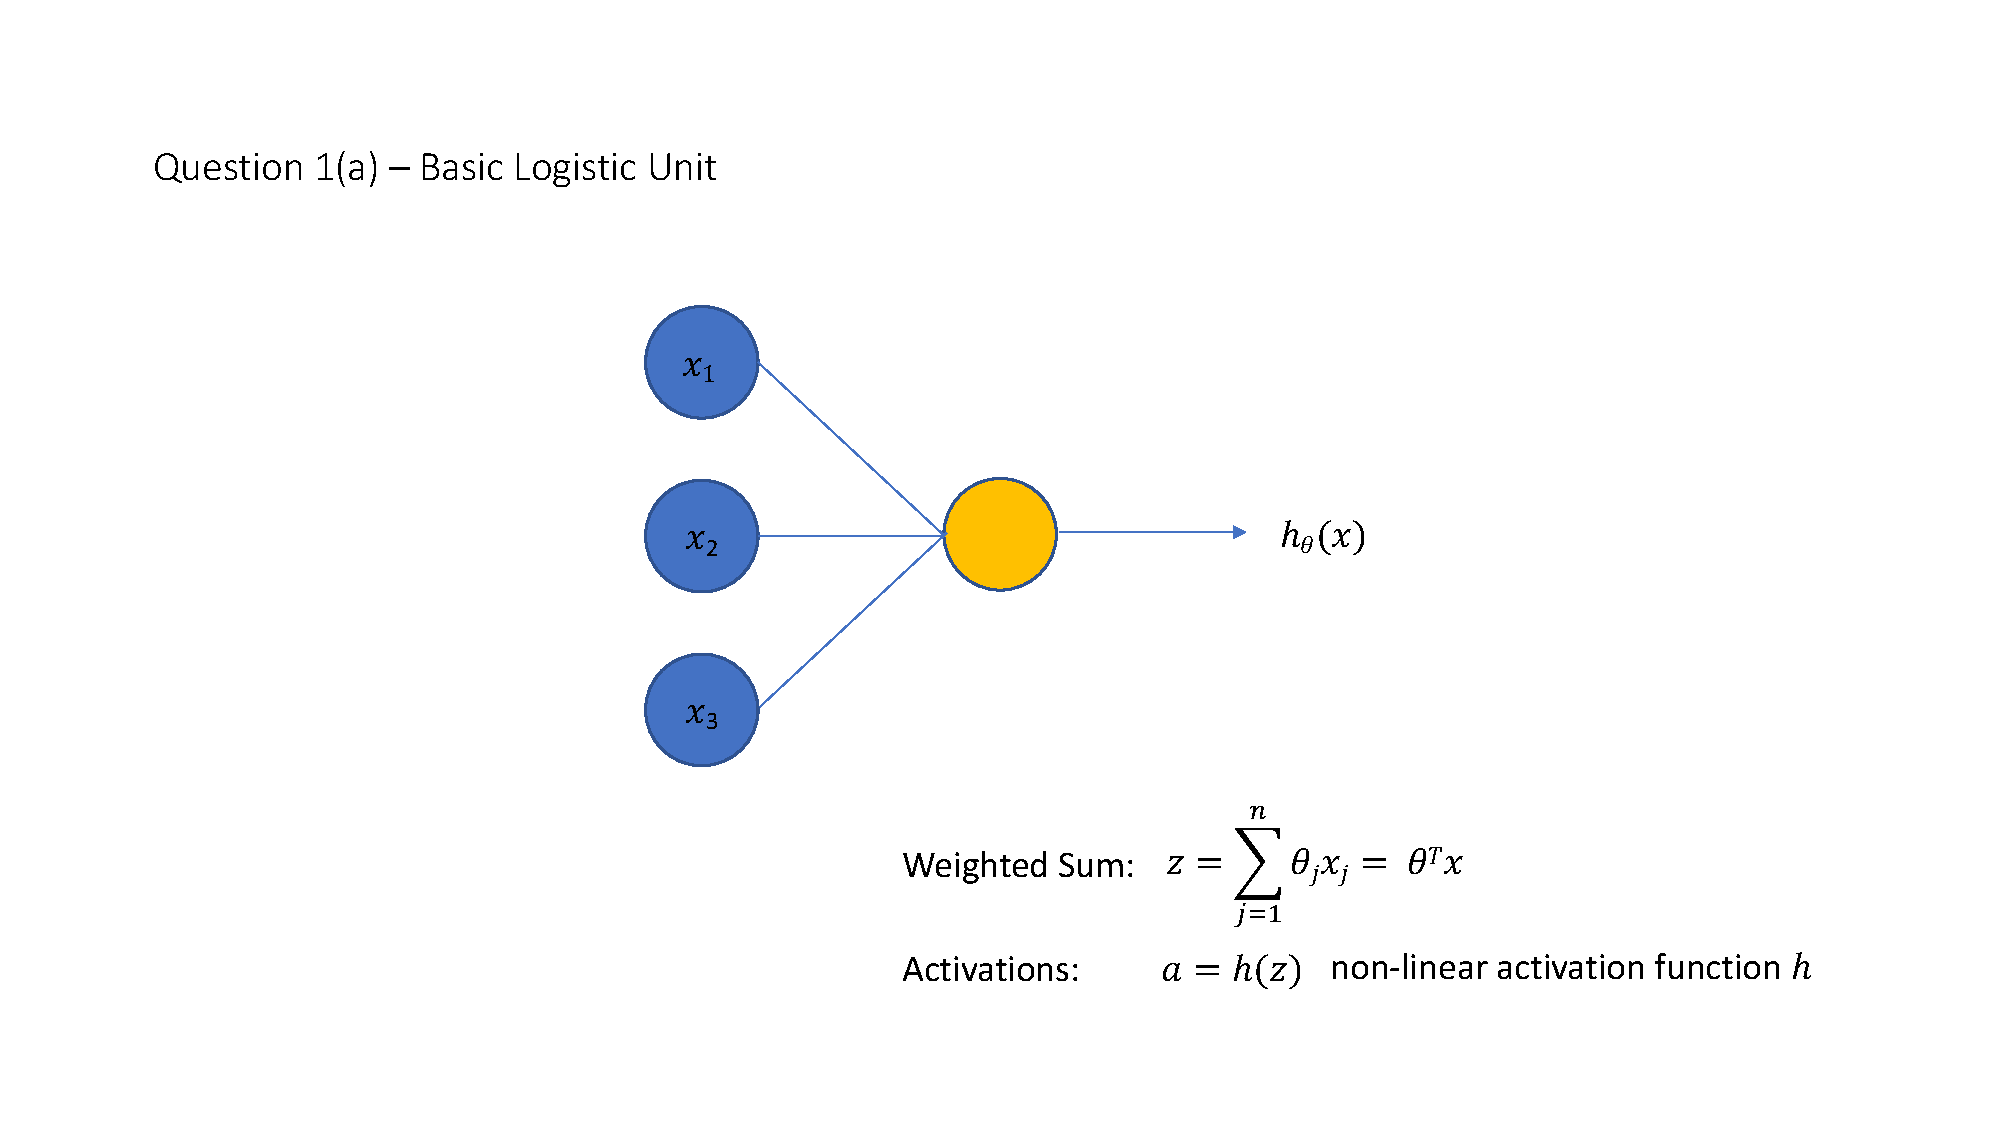
\includepdf[angle=+90]{question_1a.pdf}

% Subsection 1(c)
\subsection*{1(c)}
See diagram on following page.

% Subsection 1(d)
\subsection*{1(d)}
Consider the diagram of Question 1(c).

Firstly, consider the data transformation from the input vector $\mathbf{x}$ to the hidden layer. We now need two indices, one for the input vector elements, and one for the \emph{hidden layer} nodes. We will use $i$ for the input vector index, and $j$ for the \emph{hidden layer} nodes.

The weighted sum of the inputs at the $j^{th}$ \emph{hidden layer} node is:

\begin{equation}
z_j = \sum_{i=1}^{n}\theta_{ij} x_i
\end{equation}

where $\theta_{ij}$ is the weight between input element $i$ and \emph{hidden layer} node $j$, and $n$ is the length of the input vector $\mathbf{x}$.

Secondly, the output from each \emph{hidden layer} node is the non-linear \emph{activation function}, $h$, applied to each $z_j$:

\begin{equation}
h_{\theta j}(x) = h(z_j)
\end{equation}

 And finally, the output from the whole network, $h_\Theta(x)$ is the sum of the \emph{hidden layer} outputs:
 
\begin{equation}
h_\Theta(x) = \sum_{j=1}^{m}h_{\theta j}(x)
\end{equation}

where $m$ is the number of \emph{hidden layer} nodes.

% Subsection 1(c) - diagram
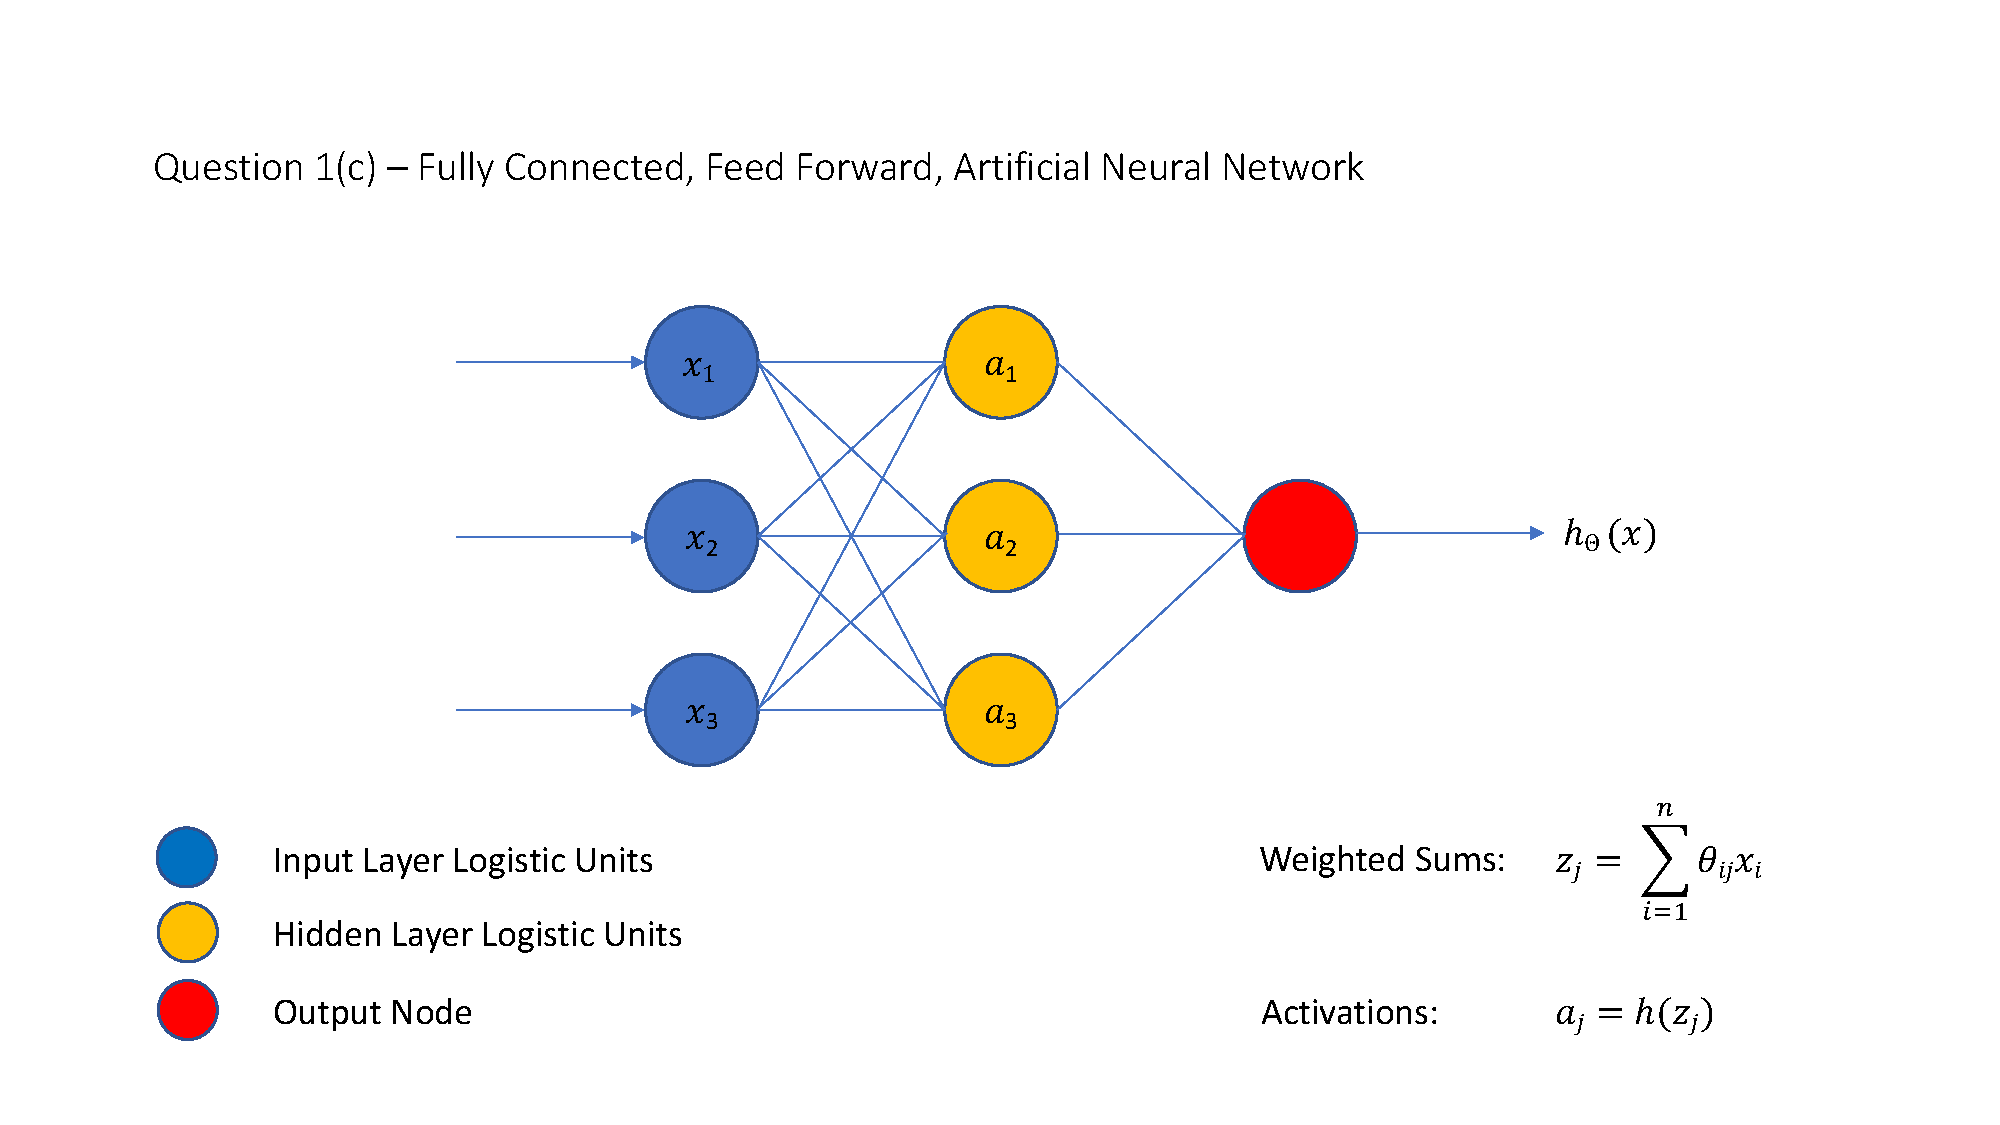
\includepdf[angle=+90]{question_1c.pdf}

% Subsection 1(e)
\subsection*{1(e)}

The cost function typically used to train neural networks for regression problems is \emph{mean square error}:

\begin{equation}
MSE(\Theta) = \frac{1}{m}\sum_{i}\sum_{j}(p_j^{(i)} - y_j^{(i)})^2
\end{equation}

The cost function typically used to train neural networks for classification problems is \emph{cross-entropy}:

\begin{equation}
C(\Theta) = -\frac{1}{m}\sum_{i}\sum_{j}y_j^{(i)}\log(p_j^{(i)})
\end{equation}

% Subsection 1(f)
\subsection*{1(f)}
Artificial Neural Networks (ANNs) are described as \emph{shallow} or \emph{deep}, and \emph{wide} or \emph{narrow}. \emph{shallow} or \emph{deep} refers to the number of layers in the network, and \emph{wide} or \emph{narrow} refers to the number of nodes in each layer.

The \emph{credit assignment path}, the CAP, of a neural network is a measure of the number of data transformations that occur as data passes through the network. For \emph{feed-forward} networks the CAP is the number of \emph{hidden layers} plus one.

A \emph{deep} neural network is generally considered to be a network with multiple layers and a CAP $>$ 2.

% Subsection 1(g)
\subsection*{1(g)}
The \emph{universal approximation theorem} states that, with appropriate parameters, single hidden layer feed-forward neural networks are \emph{universal approximators}. This means they can represent any continuous function. However, this requires an exponentially larger number of hidden layer nodes. And, training will not necessarily determine the parameters.

Deep networks provide a powerful representational framework because they have the potential to be \emph{universal approximators}, but with a limited width of hidden nodes. This makes the implementation of \emph{universal approximators} more feasible.


%
% Question 2
%
\clearpage\section*{Question 2}

% Subsection 2(a)
\subsection*{2(a)}

\emph{Gradient Descent} algorithms attempt to find the parameters $\theta$ which minimise the cost function $C(\theta)$ over the \emph{training set} using an iterative process:

\begin{equation}
\theta^{i+1} = \theta^i - \alpha\nabla_\theta C(\theta)
\end{equation}

where $\alpha$ is the \emph{learning rate}.

\emph{Batch Gradient Descent} uses the entire \emph{training set} at each iteration to calculate the gradient partial derivatives, $\nabla_\theta C(\theta)$. This produces accurate values for the partial derivatives, but is potentially slow for large \emph{training sets}.

\emph{Stochastic Gradient Descent} uses a random sub-set of the \emph{training set} at each iteration to calculate the gradient partial derivatives, $\nabla_\theta C(\theta)$. This is faster than \emph{Batch Gradient Descent}, but can produce erratic values for the partial derivatives. 

For \emph{convex} cost functions \emph{Batch Gradient Descent} will always converge to the \emph{local minima} which is also the \emph{global minima}. This is not the case for \emph{non-convex} cost functions, where \emph{local minima} are not necessarily \emph{global minima}. A bad choice of $\theta^0$ may result in \emph{Batch Gradient Descent} getting ``stuck" in a \emph{local minima}. Because the gradient partial derivatives of \emph{Stochastic Gradient Descent} are erratic, this provides a mechanism of ``jumping out of" a \emph{local minima} and improves the probability of finding the \emph{global minima}.

% Subsection 2(b)
\subsection*{2(b)}

When attempting to find the minimum of a cost function using \emph{Stochastic Gradient Descent}, the iterative process ``jumps'' around the minimum, and it is difficult to determine when a minimum has been reached. For this reason alternative optimisation algorithms are typically considered for training.

% Subsection 2(c)
\subsection*{2(c)}
Consider the iterative minimisation process: 

\begin{equation}
\theta^{i+1} = \theta^i - \alpha\nabla_\theta C(\theta)
\end{equation}

where $\alpha$ is the \emph{learning rate}.

At each step the process ``advances" towards the minimum by the step size $- \alpha\nabla_\theta C(\theta)$, which uses the \emph{current} gradient.

The \emph{Momentum Optimisation Algorithm} introduces the idea of including \emph{previous} gradients into the step size.  At each step the \emph{current} gradient is summed into a momentum term, $m$ (remember we use the negative gradient):

\begin{equation}
m^{i+1} = \beta m^i - \alpha\nabla_\theta C(\theta)
\end{equation}

The $\beta$ parameter is used to prevent the momentum getting too large, and is set between 0 and 1, typically 0.9.

The momentum $m$ is then used to update $\theta$:

\begin{equation}
\theta^{i+1} = \theta^i + m
\end{equation}

The result is that we now have an \emph{acceleration} towards the minimum.

% Subsection 2(d)
\subsection*{2(d)}

% Subsection 2(e)
\subsection*{2(e)}

% Subsection 2(f)
\subsection*{2(f)}

% Subsection 2(g)
\subsection*{2(g)}

% Subsection 2(h)
\subsection*{2(h)}


%
% Question 3
%
\clearpage\section*{Question 3}

\subsection*{3(a)}
\hl{TODO}

\subsection*{3(b)}
\hl{TODO}

\subsection*{3(c)}
\hl{TODO}

\subsection*{3(d)}
\hl{TODO}

\subsection*{3(e)}
\hl{TODO}

\subsection*{3(f)}
\hl{TODO}


%
% Question 4
%
\clearpage\section*{Question 4}

\subsection*{4(a)}
\hl{TODO}

\subsection*{4(b)}
\hl{TODO}

\subsection*{4(c)}
\hl{TODO}

\subsection*{4(d)}
\hl{TODO}

\subsection*{4(e)}
\hl{TODO}

\subsection*{4(f)}
\hl{TODO}

\begin{listing}
\inputminted[linenos]{python}{question_4f.py}
\caption{Question 4f}
\end{listing}

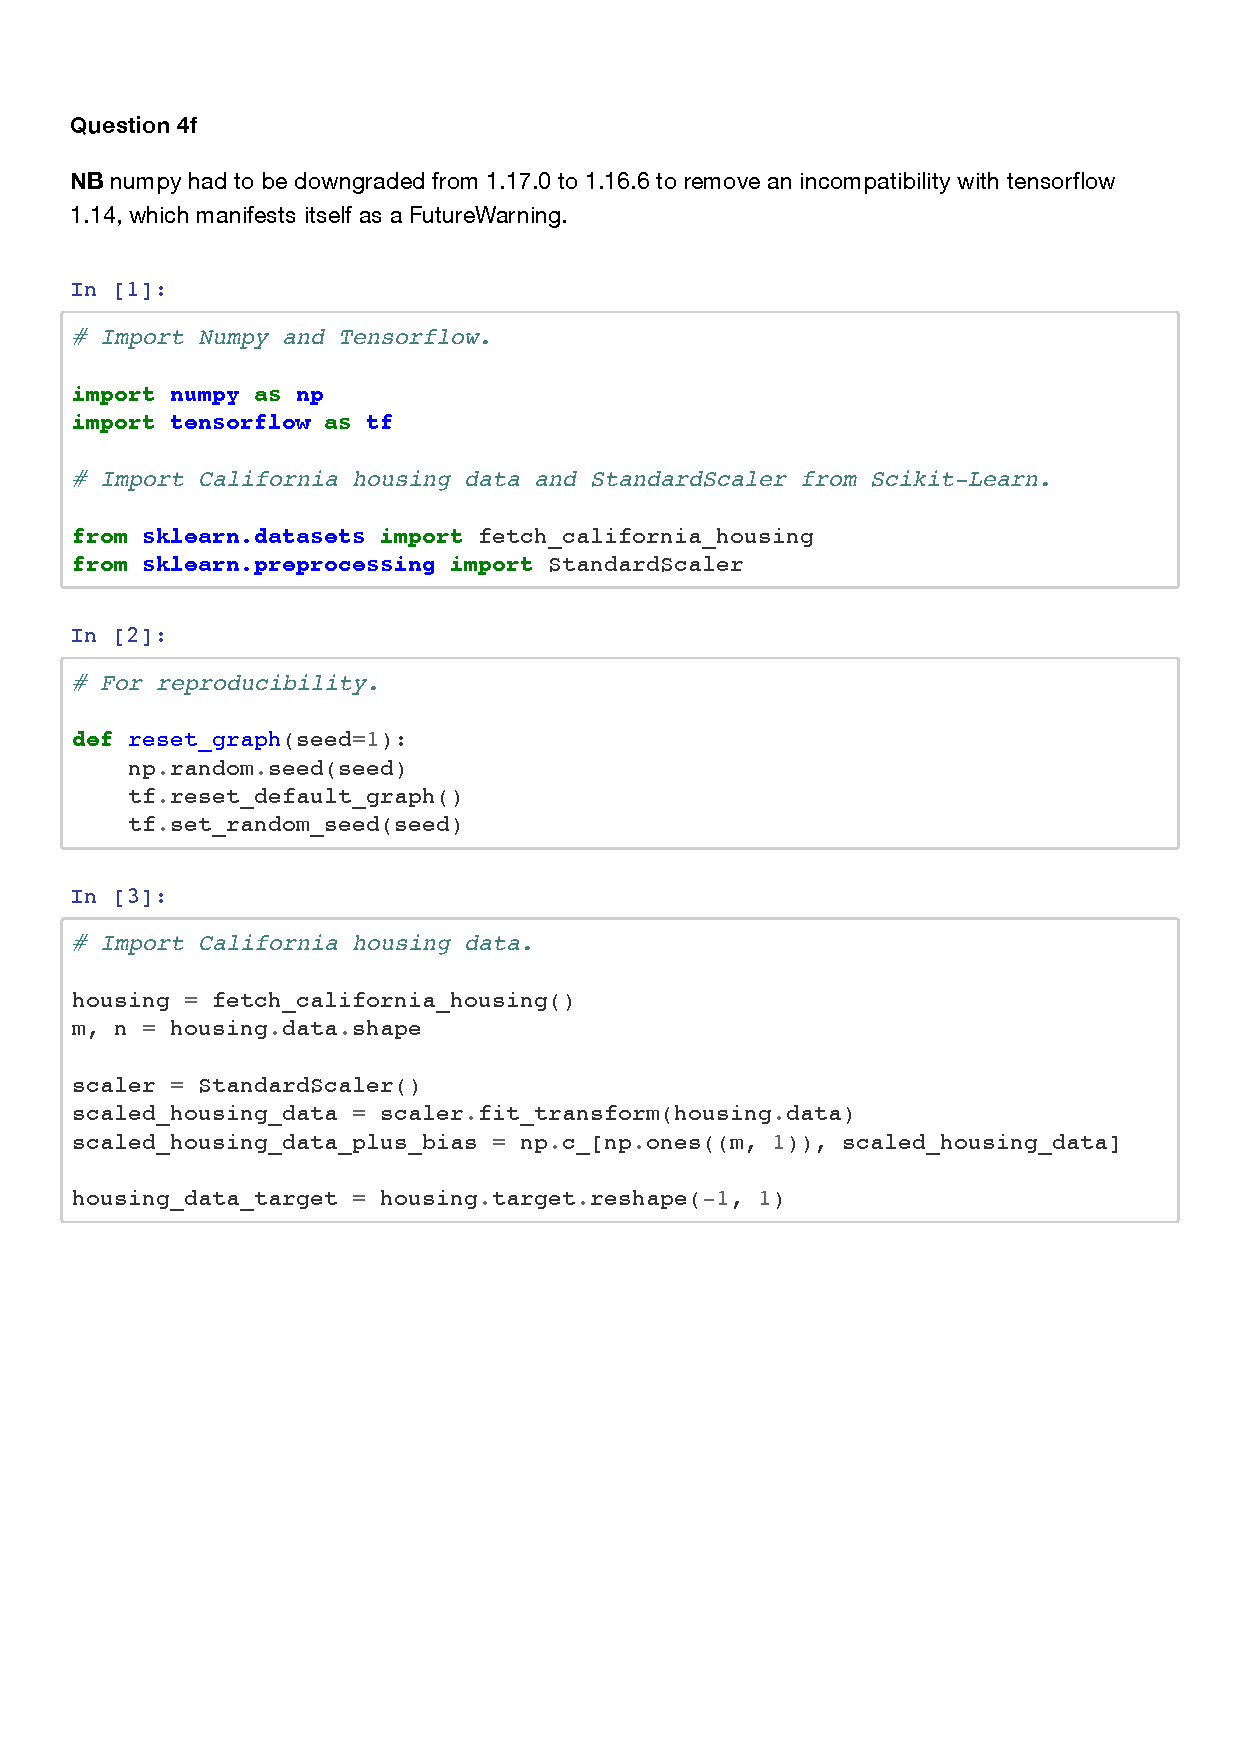
\includepdf[pages=-]{question_4f.pdf}

%
% Question 5
%
\clearpage\section*{Question 5}

\subsection*{5(a)}
\hl{TODO}

\subsection*{5(b)}
\hl{TODO}

\subsection*{5(c)}
\hl{TODO}

\subsection*{5(d)}
\hl{TODO}

\subsection*{5(e)}
\hl{TODO}

\subsection*{5(f)}
\hl{TODO}


\end{document}
